На \firef{fig:spbpu_main_bld-two-photos} приведены две картинки под~общим номером и~названием.


\begin{figure}[!htbp]
	\adjustbox{minipage=1.3em,valign=t}{\subcaption{}\label{fig:spbpu_main_bld_entrance_autumn}}%
	\begin{subfigure}[t]{\dimexpr.5\linewidth-1.3em\relax} %разрешили выделить 0,5 стр в ширину на рисунок
		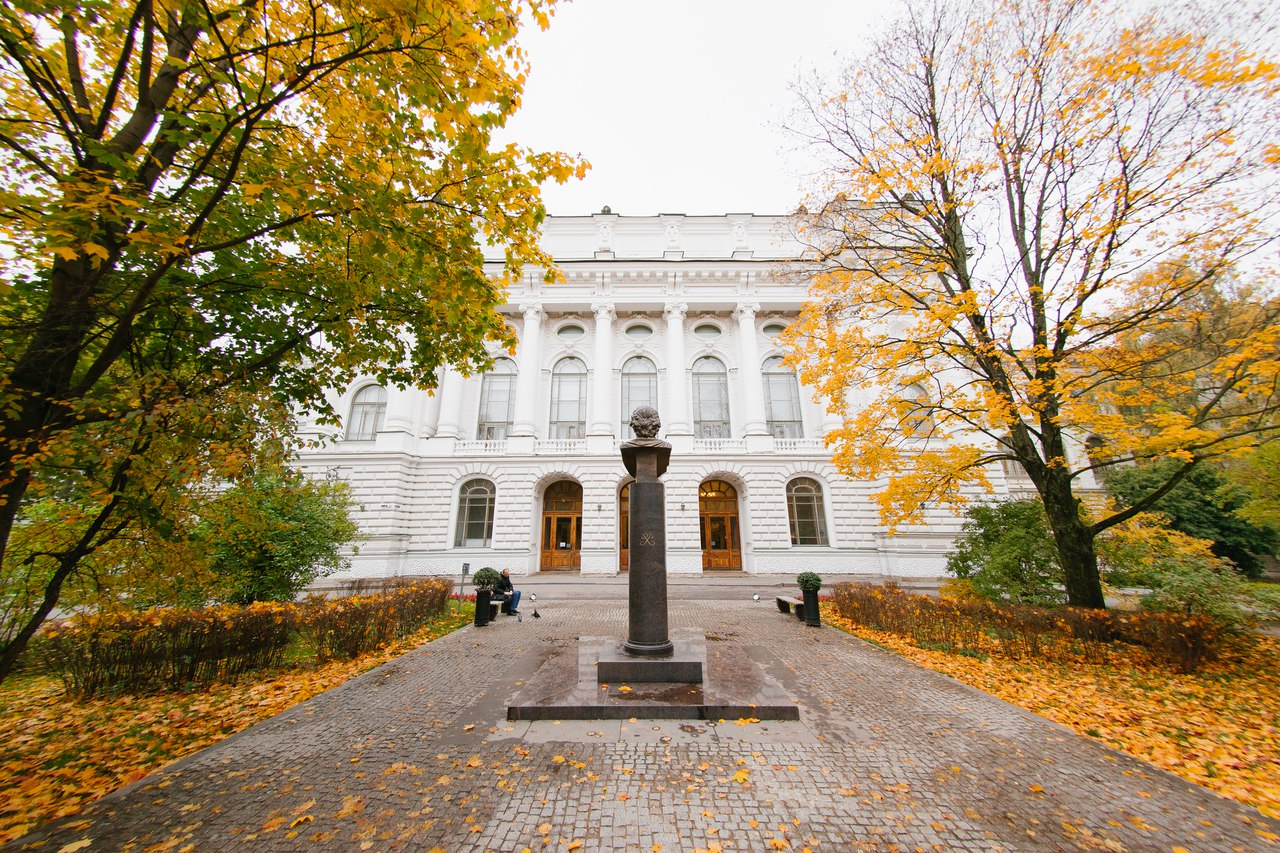
\includegraphics[height=0.20\textheight,valign=t]{my_folder/images//spbpu_main_bld_entrance_autumn} %высоту рисунка выставили как 0,3 от высоты наборного поля
	\end{subfigure}
%	\hfill %выровнять по ширине
	\adjustbox{minipage=1.3em,valign=t}{\subcaption{}\label{fig:spbpu_main_bld_whitehall}}%
	\begin{subfigure}[t]{\dimexpr.5\linewidth-1.3em\relax}%разрешили выделить 0,5 стр в ширину на рисунок
		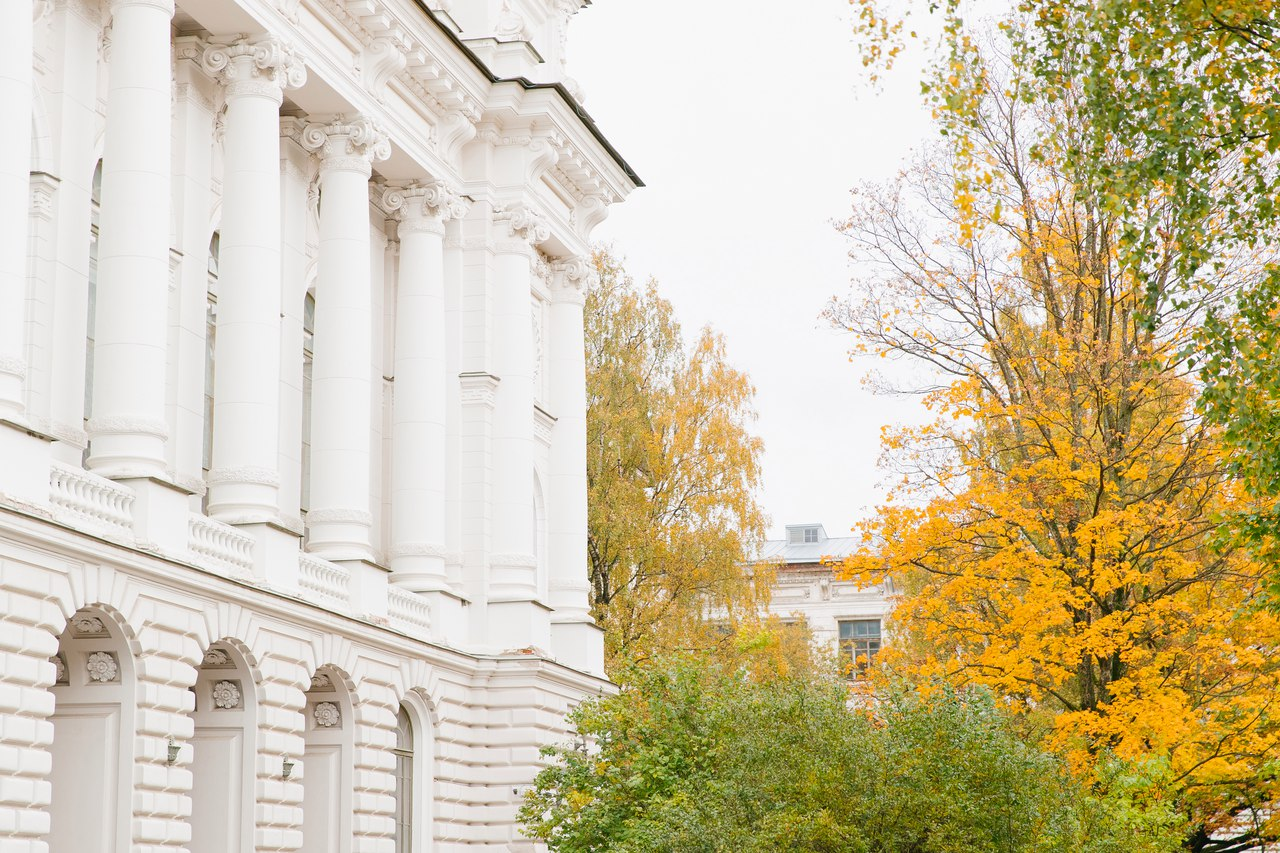
\includegraphics[height=0.20\textheight,valign=t]{my_folder/images//spbpu_main_bld_whitehall}%высоту рисунка выставили как 0,3 от высоты наборного поля
	\end{subfigure}
\captionsetup{justification=centering} %центрировать
	\caption{Вид на главное здание СПбПУ \cite{spbpu-gallery}, включая: {\itshape a} --- вход со стороны парка осенью; {\itshape b}~--- окна Белого зала}\label{fig:spbpu_main_bld-two-photos} 
\end{figure}

На \firef{fig:spbpu_main_bld_entrance_autumn} изображен вход со стороны парка СПбПУ осенью, а на \firef{fig:spbpu_main_bld_whitehall}~--- окна Белого зала.